\documentclass[12pt]{report}

\usepackage[english]{babel}
\usepackage[utf8x]{inputenc}
\usepackage{amsmath}
\usepackage{graphicx}
\usepackage{multirow}
\usepackage[hypcap]{caption}
\usepackage{setspace} 
\usepackage{float}

\title{Lab 8: Polymers}
\author{Zachary Tschirhart \\
	\small \\
        \small EID: zst75 \\
	\small Department of Aerospace Engineering and Engineering Mechanics \\
	\small \textbf{ASE 324L (Mon 2:00-5:00)} \\
	\small Unique: 13740}
\date{April 1, 2014}


\begin{document}
\maketitle

\setcounter{secnumdepth}{0}

\section{Results and Discussion}
\doublespacing

\subsection{Question 1}

The necking between the two materials is different, in strength and the area that it occurs. When the polymers begin to neck, they form stable necks. This is because the polymer chains are stretched and are aligned. The necks produced by steel and aluminum alloy do not align the carbon chains. Another difference is the strength during necking, polymers increase there strength almost exponentially at the end of their necking region. Steel and aluminum usually decrease strength toward the end of their necking region. Lastly, when the polymer specimen is unloaded, the stress-strain curve does not follow a linear back down to zero stress. The steel and aluminum specimen do follow a linear curve back to zero stress when unloaded.

\begin{equation}
  \sigma = \frac{3FL}{2bd^2}
  \label{equation:equation1}
\end{equation}

\subsection{Question 2}

\begin{figure}[H]
	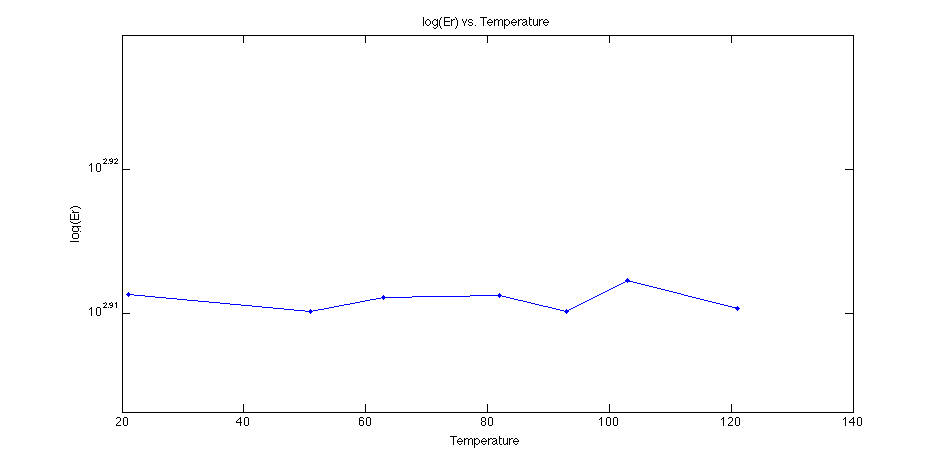
\includegraphics[width=1\textwidth]{problem2.png}
	\caption{Stress vs. strain diagrams from the eighteen specimen.}
	\label{fig:Figure1}
\end{figure}

\subsection{Question 3}

\subsection{Question 4}

\subsection{Question 5}

\subsection{Question 6}

\end{document}
